
%Abstract of architecture
In this report, the implementation of a neural network capable of recognizing human handwriting on an FPGA will be analyzed. \\
To achieve this, the FPGA is connected to a touchscreen LCD display, where the user can write. \\
The hardware components used for this project are:

\begin{itemize}
    \item \textbf{DE10-lite dev. board}:\\
    Is a development board, produced by \terasic that contains an Altera MAX10 FPGA and other useful peripherals like: button, switch, seven-segment displays, SDRAM and flash memory, etc.
    \item \textbf{LT24 Touch LCD Display}:\\
    Is a daughter board produced by \terasic that connects with the GPIO pins of the \textbf{DE10-lite} board and allow the communication between the FPGA and the LT24 LCD display.
\end{itemize}

\subsection{Altera DE10-lite dev. board}

The DE10-Lite is a low-cost FPGA development board based on the Intel (Altera) MAX10 device. \\
It is designed for system-level prototyping and is suitable for applications in the industrial, automotive, and consumer fields. \\
It provides a range of useful peripherals:

\begin{multicols}{2}
    \begin{itemize}
        \setlength\itemsep{0pt}
        \setlength\parskip{0pt}
        \item USB-Blaster interface
        \item 64 MB SDRAM
        \item On-board flash memory
        \item Accelerometer
        \item Ambient light sensor
        \item VGA output interface
        \item GPIO header
        \item 7-segment display
        \item User LEDs
        \item Slide switches
        \item Push buttons
        \item On-board clock oscillator
    \end{itemize}
\end{multicols}

\begin{figure}[h!]
    \centering
    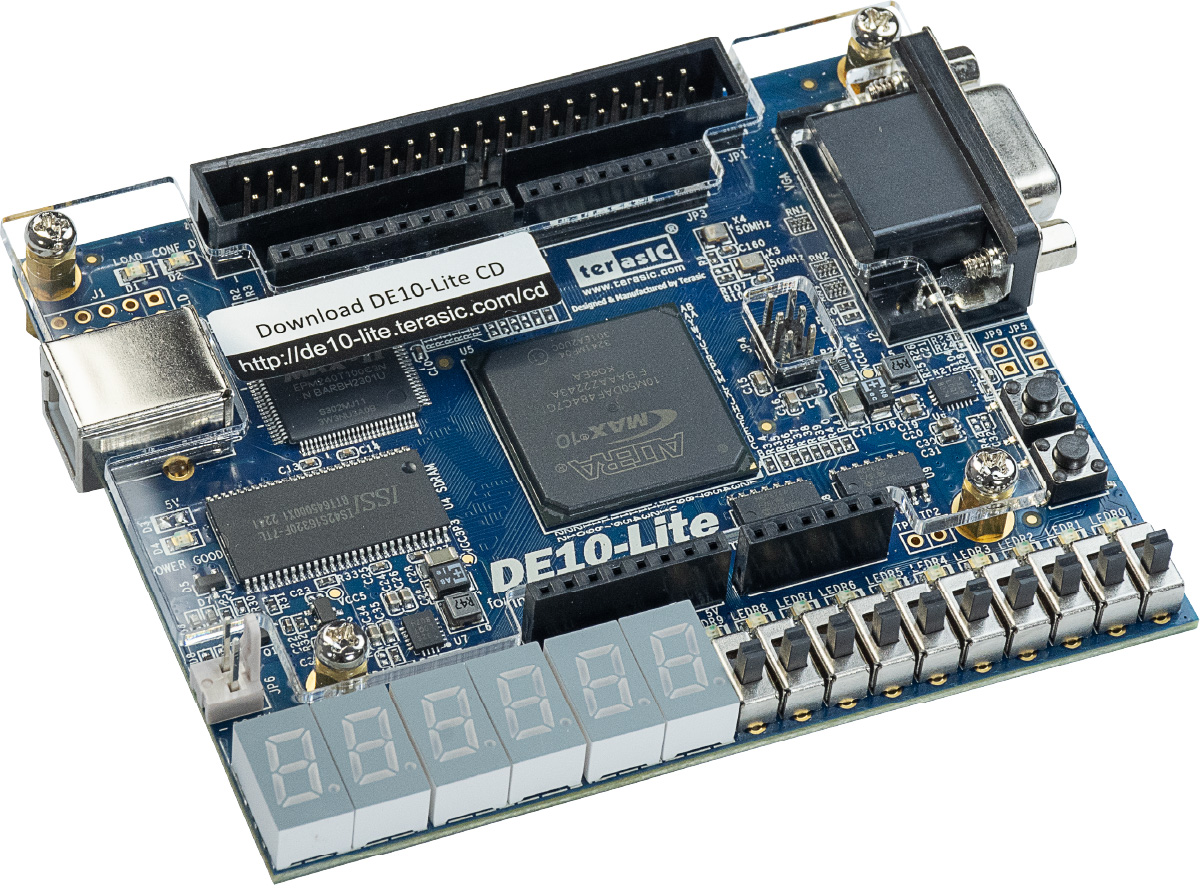
\includegraphics[width=0.5\linewidth]{img/DE10-Lite_45.jpg}
    \caption{DE10 lite dev. board}
    \label{fig:DE10-Lite_45}
\end{figure}

\newpage
\subsection{Overview of the LCD Display Used}

\begin{figure}[h!]
    \centering
    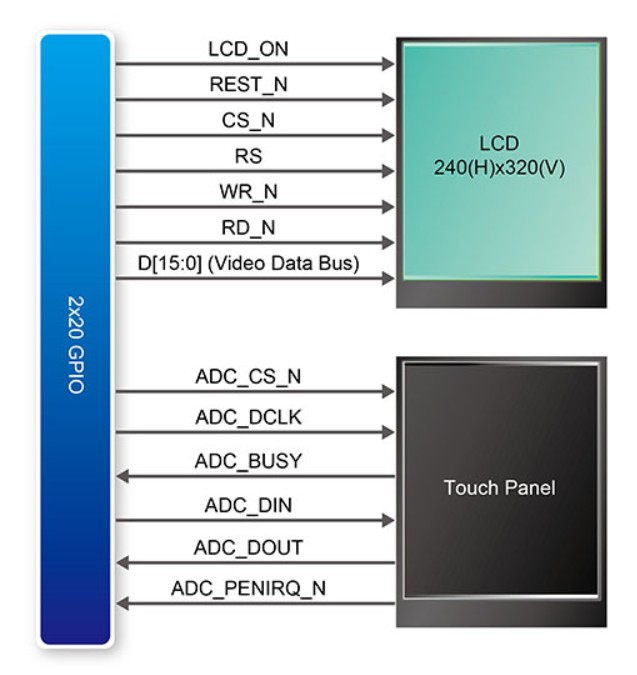
\includegraphics[width=0.5\linewidth]{img/LCD_block_diagram.jpg}
    \caption{LT24 LCD Display block diagram}
    \label{fig:LCD_block_diagram}
\end{figure}

\noindent
The LT24 LCD module integrates both a display panel and a resistive touch screen, which are interfaced using two different communication protocols. \
The touch panel uses an SPI interface to communicate with the AD7843 ADC integrated inside the module. \\
This device converts the analog touch coordinates into digital values, which are then read by the FPGA through the SPI bus. \\
The LCD panel is driven through a parallel bus interface, which is used to transmit pixel data for image rendering. \\
This interface allows the FPGA to directly write image data to the display for real-time visualization.

\newpage
\subsection{Fully connected Neural Network}

A fully connected neural network is a structure composed of basic elements called \textbf{neurons}, which are interconnected.

\vspace{1em}
\begin{figure}[h!]

    \begin{center}
        \resizebox{0.8\linewidth}{!}{
            \begin{tcolorbox}[neuralbox, width=0.95\linewidth]
            
                \centering
                
                \begin{neuralnetwork}[height=7.5]
                
                    \newcommand{\x}[2]{$x_#2$}
                    \newcommand{\y}[2]{$\hat{y}_#2$}
                    \newcommand{\hfirst}[2]{\small $h^{(1)}_#2$}
                    \newcommand{\hsecond}[2]{\small $h^{(2)}_#2$}
                
                    \inputlayer[count=3, bias=false, title=Input\\layer, text=\x]
                
                    \hiddenlayer[count=7, bias=false, title=Hidden\\layer 1, text=\hfirst]
                    \linklayers
                
                    \hiddenlayer[count=6, bias=false, title=Hidden\\layer 2, text=\hsecond]
                    \linklayers
                
                    \outputlayer[count=2, title=Output\\layer, text=\y]
                    \linklayers
                
                \end{neuralnetwork}
            
            \end{tcolorbox}
        }

    \end{center}

    \caption{Fully connected Deep Neural Network with two hidden layers}
    \label{fig:nn_architecture}

\end{figure}

\noindent
As shown in \autoref{fig:nn_architecture}, neurons are arranged in different layers; the output of the neurons in one layer becomes the input to the neurons in the next layer. \\
The first layer is called the \textbf{input layer}, and its inputs correspond to the inputs of the neural network to be processed. \\
The last layer is called the \textbf{output layer}, and its output represents the final processed output of the neural network. \\
The intermediate layers are called \textbf{hidden layers} and may not be present in some networks. \\
Networks with at least one hidden layer are referred to as deep neural networks.

\newpage
\subsubsection{Neuron structure}
To understand the behavior of a neural network, we must analyze the structure of a single neuron. 

\begin{figure}[h!]

    \begin{center}
    
        \begin{tikzpicture}[
            neuron/.style={circle, draw, minimum size=8mm, fill=green!30},
            weight/.style={rectangle, draw, minimum size=6mm, fill=purple!30},
            sum/.style={circle, draw, minimum size=10mm, fill=gray!15},
            act/.style={rectangle, draw, minimum size=8mm, fill=orange!30},
            output/.style={circle, draw, minimum size=8mm, fill=red!30},
            bias/.style={circle, draw, minimum size=8mm, fill=blue!30},
            arrow/.style={-{Stealth}, thick}
        ]
            
            % INPUTS
            \node[neuron] (x1) at (0,2) {$x_1$};
            \node[neuron] (x2) at (0,1) {$x_2$};
            \node (vdots) at (0,0) {$\vdots$};
            \node[neuron] (xn) at (0,-1) {$x_n$};
            
            % WEIGHTS
            \node[weight] (w1) at (2,2) {$w_1$};
            \node[weight] (w2) at (2,1) {$w_2$};
            \node (wdots) at (2,0) {$\vdots$};
            \node[weight] (wn) at (2,-1) {$w_n$};
            
            % SUM
            \node[sum] (s) at (4,0.5) {$\Sigma$};
        
            % OUTPUT
            \node[output] (a) at (8,0.5) {$a$};
        
            % BIAS
            \node[bias] (b) at (4,2) {$b$};
            
            % ACTIVATION FUNCTION
            \node[act] (phi) at (6,0.5) {$\phi(\bullet)$};
            
            % CONNECTIONS input -> weights
            \draw[arrow] (x1) -- (w1);
            \draw[arrow] (x2) -- (w2);
            \draw[arrow] (xn) -- (wn);
            
            % CONNECTIONS weights -> sum
            \draw[arrow] (w1) -- (s);
            \draw[arrow] (w2) -- (s);
            \draw[arrow] (wn) -- (s);
        
            % BIAS (from top)
            \draw[arrow] (b) -- (s);
            
            % SUM -> ACTIVATION (with z label)
            \draw[arrow] (s) -- (phi)
                node[midway, above] {$z$};
            
            % ACTIVATION -> OUTPUT
            \draw[arrow] (phi) -- (a);
        
        \end{tikzpicture}

    \end{center}

    \caption{Neuron block diagram structure}
    \label{fig:neuron_structure}

\end{figure}

\noindent
As we can see in \autoref{fig:neuron_structure}, a neuron is a basic computational unit that processes input data to produce an output following the \cref{eq:neuron_math_formula}

\begin{equation}
    \begin{cases}
        z_j &= \sum_i w_{ij} \cdot x_i + b_j \\
        a_j &= \phi(z_j)
    \end{cases}
    \label{eq:neuron_math_formula}
\end{equation}

\noindent
where:

\begin{itemize}
    \setlength\itemsep{0pt}
    \setlength\parskip{0pt}
    \item \(w_{ij}\): Weight of the j-th neuron associated to the i-th input
    \item \(x_i\): i-th input of the j-th neuron
    \item \(b_j\): bias of the j-th neuron
    \item \(z_j\): weighted sum of the j-th neuron
    \item \(\phi(\bullet)\): activation function of the j-th neuron
\end{itemize}

\noindent
The goal of using a neural network is to choose the correct values for the weights and biases of all neurons in order to obtain the desired output. \\
The process of choosing the weights and biases of the neurons is called the \textbf{Training process}. \\
The process of feeding inputs into the network to obtain its output is called the \textbf{Inference process}.

\newpage
\subsubsection{Inference Process}

For a neural network, the inference process consist on computing the output of every neuron and give them as input of the neuron of the next layer of the network. \\
To simplify the computation process the inputs and the outputs are stored in a vector and the weights are stored into matrix like is shown in \cref{eq:inf_matrix}.

\begin{equation}
    \begin{bmatrix}
        z_1 & \cdots & z_n
    \end{bmatrix}
    = 
    \begin{bmatrix}
        x_1 & \cdots & x_m
    \end{bmatrix} 
    \begin{bmatrix}
        w_{11} & \cdots & w_{1n} \\
        \vdots & \ddots & \vdots \\
        w_{m1} & \cdots & w_{mn}
    \end{bmatrix}
    +
    \begin{bmatrix}
        b_1 & \cdots & b_n
    \end{bmatrix}
    \label{eq:inf_matrix}
\end{equation}

\noindent
where:

\begin{itemize}
    \setlength\itemsep{0pt}
    \setlength\parskip{0pt}
    \item n: is the number of outputs of the network
    \item m: is the number of inputs of the network
\end{itemize}

\noindent
To obtain the output of a neuron layer, the weighted sum vector must pass through the activation function, like is shown in \cref{eq:act_funct}.

\begin{equation}
    \begin{bmatrix}
        a_1 & \cdots & a_n
    \end{bmatrix}
    = 
    \begin{bmatrix}
        \phi(z_1) & \cdots & \phi(z_n)
    \end{bmatrix}
    \label{eq:act_funct}
\end{equation}

\noindent
The activation functions can be various, but the most common ones are shown in \autoref{fig:activation_funct}

\begin{figure}[h!]
    \begin{center}
        \begin{tabular}{cc}
            
            % SIGMOID
            \begin{minipage}{0.45\textwidth}
                \centering
                \textbf{Sigmoid} $\sigma(x)$
                
                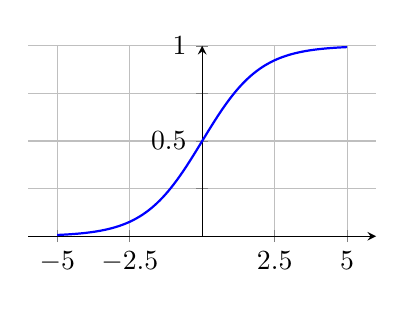
\begin{tikzpicture}
                    \begin{axis}[
                        width=6cm,
                        height=4cm,
                        axis lines=middle,
                        xmin=-6, xmax=6,
                        ymin=0, ymax=1,
                        xtick = {-5, -2.5, 0, 2.5, 5},
                        xticklabels = { $-5$, $-2.5$, $0$, $2.5$, $5$},
                        ytick = {0, 0.25, 0.5, 0.75, 1},
                        yticklabels = {$0$, , $0.5$, , $1$},
                        samples=100,
                        grid=both,
                    ]
                        \addplot[blue, thick] {1/(1+exp(-x))};
                    \end{axis}
                \end{tikzpicture}
            \end{minipage}
            
            &
            
            % TANH
            \begin{minipage}{0.45\textwidth}
                \centering
                \textbf{Tanh} $\tanh(x)$
                
                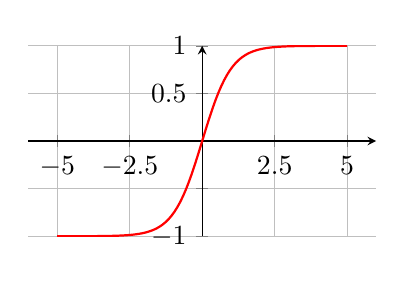
\begin{tikzpicture}
                    \begin{axis}[
                        width=6cm,
                        height=4cm,
                        axis lines=middle,
                        xmin=-6, xmax=6,
                        ymin=-1, ymax=1,
                        xtick = {-5, -2.5, 0, 2.5, 5},
                        xticklabels = { $-5$, $-2.5$, $0$, $2.5$, $5$},
                        ytick = {-1, -0.5, 0, 0.5, 1},
                        yticklabels = {$-1$, , $0$, $0.5$, $1$},
                        samples=100,
                        grid=both,
                    ]
                        \addplot[red, thick] {tanh(x)};
                    \end{axis}
                \end{tikzpicture}
            \end{minipage}
            
            \\[1em]
            
            % RELU
            \begin{minipage}{0.45\textwidth}
                \centering
                \textbf{ReLU}
                
                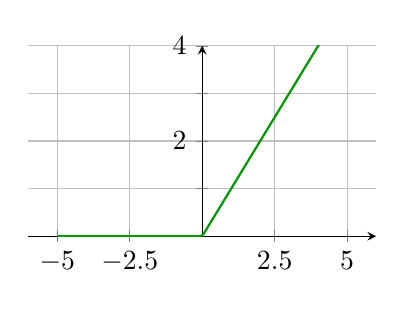
\begin{tikzpicture}
                    \begin{axis}[
                        width=6cm,
                        height=4cm,
                        axis lines=middle,
                        xmin=-6, xmax=6,
                        ymin=0, ymax=4,
                        xtick = {-5, -2.5, 0, 2.5, 5},
                        xticklabels = { $-5$, $-2.5$, $0$, $2.5$, $5$},
                        ytick = {0, 1, 2, 3, 4},
                        yticklabels = {$0$, , $2$, , $4$},
                        samples=100,
                        grid=both,
                    ]
                        \addplot[green!60!black, thick] {max(0,x)};
                    \end{axis}
                \end{tikzpicture}
            \end{minipage}
            
            &
            
            % LEAKY RELU
            \begin{minipage}{0.45\textwidth}
                \centering
                \textbf{Leaky ReLU}
                
                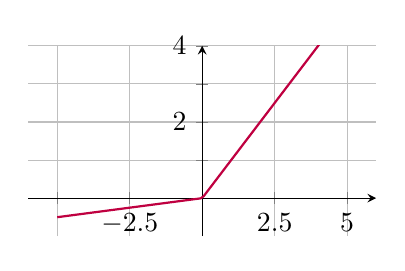
\begin{tikzpicture}
                    \begin{axis}[
                        width=6cm,
                        height=4cm,
                        axis lines=middle,
                        xmin=-6, xmax=6,
                        ymin=-1, ymax=4,
                        xtick = {-5, -2.5, 0, 2.5, 5},
                        xticklabels = { , $-2.5$, $0$, $2.5$, $5$},
                        ytick = {0, 1, 2, 3, 4},
                        yticklabels = {$0$, , $2$, , $4$},
                        samples=100,
                        grid=both,
                    ]
                        \addplot[purple, thick] {x > 0 ? x : 0.1*x};
                    \end{axis}
                \end{tikzpicture}
            \end{minipage}
            
        \end{tabular}
    \end{center}

    \caption{Most common activation functions}
    \label{fig:activation_funct}

\end{figure}

\subsubsection{Training Process}

During the training process, we need to send some inputs to the network and compare the obtained outputs with the desired ones. \\
Then, the weights and biases of the network must be modified to get closer to the desired output. \\
To train the network, an error function called the \textbf{cost function} is defined. This function represents the difference between the expected output of the network and the actual output, depending on the weights and biases of the network. \\
The goal of the training process is to choose the values of the weights and biases that minimize the cost function. \\
There are different types of cost functions, but the most common one is the quadratic cost function, defined in \cref{eq:quadratic_cost_funct}

\begin{equation}
    C(\vec{w},\vec{b}) = \frac{ || \vec{y} - \vec{a}_{\text{out layer}} || ^ 2 }{2}
    \label{eq:quadratic_cost_funct}
\end{equation}

\noindent
where:

\begin{itemize}
    \setlength\itemsep{0pt}
    \setlength\parskip{0pt}
    \item \(\vec{w}\): is the weight vector
    \item \(\vec{b}\): is the bias vector
    \item \(\vec{a}_{\text{out layer}}\): is the output vector
    \item \(\vec{y}\): is the desired output vector
\end{itemize}

\noindent
If we consider small changes in the weights and biases, we can approximate the variation of the cost function as

\[
    \Delta C \sim \vec{\nabla} C \cdot \Delta (\vec{w}, \vec{b})
\]

\noindent
where

\[
    \vec{\nabla} C = \left( \frac{\partial C}{\partial w_1}, \cdots, \frac{\partial C}{\partial w_{m \cdot n}}, \frac{\partial C}{\partial b_1}, \cdots, \frac{\partial C}{\partial b_n} \right)
\]

\noindent
We start with random values for the weights and biases of the network. \\
Then, each time we send an input to the network, we compute the gradient of the cost function and update the weights and biases to reduce the value of the cost function. \\
If we update the weight and bias vectors as shown in \cref{eq:update_weight_bias}

\begin{equation}
    \Delta (\vec{w}, \vec{b}) = - \eta \vec{\nabla} C
    \label{eq:update_weight_bias}
\end{equation}

\noindent
we obtain an always negative variation of the cost function (according to the approximation above) until we reach its minimum value. In fact,

\[
    \Delta C \sim \vec{\nabla} C \cdot \Delta (\vec{w}, \vec{b}) = - \eta 
    || \vec{\nabla} C || ^ 2 < 0 
\]

\noindent
There are various types of cost functions, but the important property is that every function used must have a minimum when \(\vec{y} = \vec{a}_{\text{out layer}}\). \\
It is easy to verify that the quadratic cost function satisfies this property, since it is a paraboloid.